\documentclass[12pt, a4paper]{report}
\usepackage{geometry}
\usepackage{graphicx}
\usepackage{hyperref}
\usepackage{titlesec}
\usepackage{tocloft}
\usepackage{tikz}
\usetikzlibrary{shapes.geometric, arrows.meta}

\geometry{margin=1in}

\hypersetup{
    colorlinks=true,
    linkcolor=black,
    filecolor=magenta,      
    urlcolor=blue,
}

\titleformat{\chapter}[display]
  {\normalfont\bfseries}{}{0pt}{\Huge}

\begin{document}

% -------------------------------------------------------------------
% 1. Title Page
% -------------------------------------------------------------------
\begin{titlepage}
    \centering
    \vspace*{2cm}
    
    {\Huge \textbf{eDirectory}}
    
    \vspace{0.5cm}
    {\Large \textit{A Community-Based Social \& Live Streaming Platform}}
    
    \vspace{3cm}
    
    {\Large \textbf{Prepared by:}} \\
    \vspace{0.2cm}
    {\Large Development Team}
    
    \vspace{2cm}
    
    {\Large \today}
    
    \vfill
\end{titlepage}

% -------------------------------------------------------------------
% 2. Abstract
% -------------------------------------------------------------------
\chapter*{Abstract}
eDirectory is a comprehensive mobile application designed to foster closed-community interactions through a unique blend of directory services, social networking, and live streaming aggregation. The platform connects organizations with users, allowing for verified content distribution, role-based management, and real-time engagement. By integrating features such as a "Mini Facebook" social feed, live video link aggregation from major platforms (YouTube, Facebook), and a detailed organizational directory, eDirectory serves as a centralized hub for community communication and activity. This document details the architectural design, functional capabilities, and technical specifications of the eDirectory system.

\tableofcontents

% -------------------------------------------------------------------
% 3. Introduction
% -------------------------------------------------------------------
\chapter{Introduction}

\section{Problem Statement}
In an era of fragmented digital communication, communities often struggle to maintain a centralized and verified channel for interaction. Standard social media platforms can be noisy and unmoderated, while traditional directory apps lack dynamic engagement features. There is a need for a unified platform that combines the structure of a directory with the engagement of a social network, tailored for specific communities or organizations.

\section{Motivation}
The motivation behind eDirectory is to empower communities to create their own digital ecosystem. By providing tools for organizations to broadcast content (live streams, posts) and for users to interact meaningfully (likes, comments, shares, follows), eDirectory bridges the gap between static information and dynamic social interaction.

\section{Objectives}
\begin{itemize}
    \item To provide a secure, role-based platform for community management.
    \item To aggregate live streaming content from external providers into a central "Live Wall."
    \item To facilitate social networking within a controlled, verified environment.
    \item To offer a comprehensive directory of organizations with detailed profiles.
\end{itemize}

% -------------------------------------------------------------------
% 4. System Overview
% -------------------------------------------------------------------
\chapter{System Overview}
The eDirectory application functions as a "closed-community" ecosystem. It is designed to be deployed for specific groups, associations, or networks where verifying the identity of organizations and users is crucial. The system revolves around three core pillars: The Directory (information), The Social Feed (engagement), and The Live Wall (real-time events).

\section{Closed-Community Concept}
Access to the platform is regulated. Unlike open social networks, eDirectory emphasizes verification. Organizations must be approved by administrators, ensuring that the directory remains trustworthy and relevant to the community.

\section{Role-Based Access Control}
The system enforces strict data separation and feature access based on user roles, ensuring that administrative functions are protected and user experiences are tailored to their status.

% -------------------------------------------------------------------
% 5. User Roles and Permissions
% -------------------------------------------------------------------
\chapter{User Roles and Permissions}

\section{Super Admin}
The highest level of authority in the system.
\begin{itemize}
    \item \textbf{Responsibilities:} System oversight, organization approval/rejection, user management, and content moderation.
    \item \textbf{Access:} Full access to all backend data and administrative dashboards.
\end{itemize}

\section{Organization}
Entities that provide content and services within the directory.
\begin{itemize}
    \item \textbf{Responsibilities:} Managing their public profile, posting live stream links, creating social posts, and interacting with followers.
    \item \textbf{Access:} Organization dashboard, profile editing, post creation, live link submission.
\end{itemize}

\section{User}
General members of the community.
\begin{itemize}
    \item \textbf{Responsibilities:} Consuming content, following organizations, participating in live events, and engaging socially.
    \item \textbf{Access:} Home feed, directory search, live wall, personal profile management.
\end{itemize}

% -------------------------------------------------------------------
% 6. Functional Requirements
% -------------------------------------------------------------------
\chapter{Functional Requirements}

\section{Authentication \& Approval Flow}
\begin{itemize}
    \item Secure email/password login and registration.
    \item Mandatory approval workflow for Organization accounts before they go public.
    \item Secure session management and token-based authentication.
\end{itemize}

\section{Organization Directory}
\begin{itemize}
    \item Searchable and filterable list of all approved organizations.
    \item Detailed profile pages displaying contact info, location, and historical posts.
    \item "Follow" functionality for users to subscribe to updates.
\end{itemize}

\section{Live Streaming Links}
\begin{itemize}
    \item Organizations can post URLs to live streams hosted on YouTube or Facebook.
    \item The system validates these links and embeds them in the "Live Wall."
    \item Real-time "LIVE" badges and notifications for active streams.
\end{itemize}

\section{Notifications}
\begin{itemize}
    \item Push notifications for new live streams from followed organizations.
    \item In-app alerts for social interactions (likes, comments).
\end{itemize}

\section{Social Networking}
\begin{itemize}
    \item A rich media feed supporting text and image posts.
    \item Interactions: Likes, Comments, and Shares.
    \item User-to-User and User-to-Organization connectivity.
\end{itemize}

% -------------------------------------------------------------------
% 7. Non-Functional Requirements
% -------------------------------------------------------------------
\chapter{Non-Functional Requirements}

\section{Security}
Data transit is encrypted via SSL/TLS. User passwords are hashed. Sensitive API endpoints are protected by role-based middleware.

\section{Scalability}
The backend is built on serverless, scalable infrastructure (Firebase) capable of handling concurrent users and data spikes during live events.

\section{Performance}
The Flutter-based frontend ensures native performance on both iOS and Android (60fps rendering). Image caching strategies are employed to minimize bandwidth usage.

\section{Usability}
The UI is designed with a "Warm Palette" aesthetic, prioritizing accessibility and ease of navigation.

\section{Maintainability}
The codebase follows Clean Architecture principles, ensuring separation of concerns and ease of future updates.

% -------------------------------------------------------------------
% 8. Application Flow
% -------------------------------------------------------------------
\chapter{Application Flow}

\section{User Registration Flow}

\begin{figure}[h]
\centering
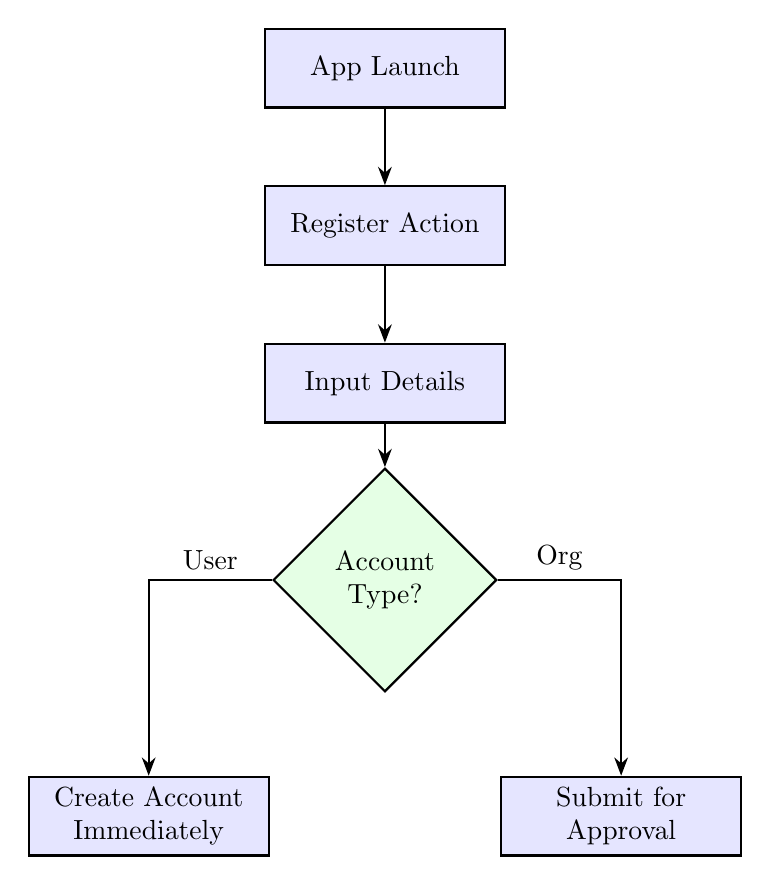
\begin{tikzpicture}[node distance=2cm, auto,
  process/.style={rectangle, draw=black, thick, fill=blue!10, text width=8em, text centered, minimum height=1cm},
  decision/.style={diamond, draw=black, thick, fill=green!10, text width=6em, text centered, inner sep=0pt},
  arrow/.style={thick, ->, >=Stealth}
]

\node (launch) [process] {App Launch};
\node (register) [process, below of=launch] {Register Action};
\node (input) [process, below of=register] {Input Details};
\node (decide) [decision, below of=input, yshift=-0.5cm] {Account Type?};
\node (user) [process, below of=decide, xshift=-3cm, yshift=-1cm] {Create Account Immediately};
\node (org) [process, below of=decide, xshift=3cm, yshift=-1cm] {Submit for Approval};

\draw [arrow] (launch) -- (register);
\draw [arrow] (register) -- (input);
\draw [arrow] (input) -- (decide);
\draw [arrow] (decide) -| node[near start, above] {User} (user);
\draw [arrow] (decide) -| node[near start, above] {Org} (org);

\end{tikzpicture}
\caption{User Registration Flow Diagram}
\end{figure}

\section{Approval Workflow}

\begin{figure}[h]
\centering
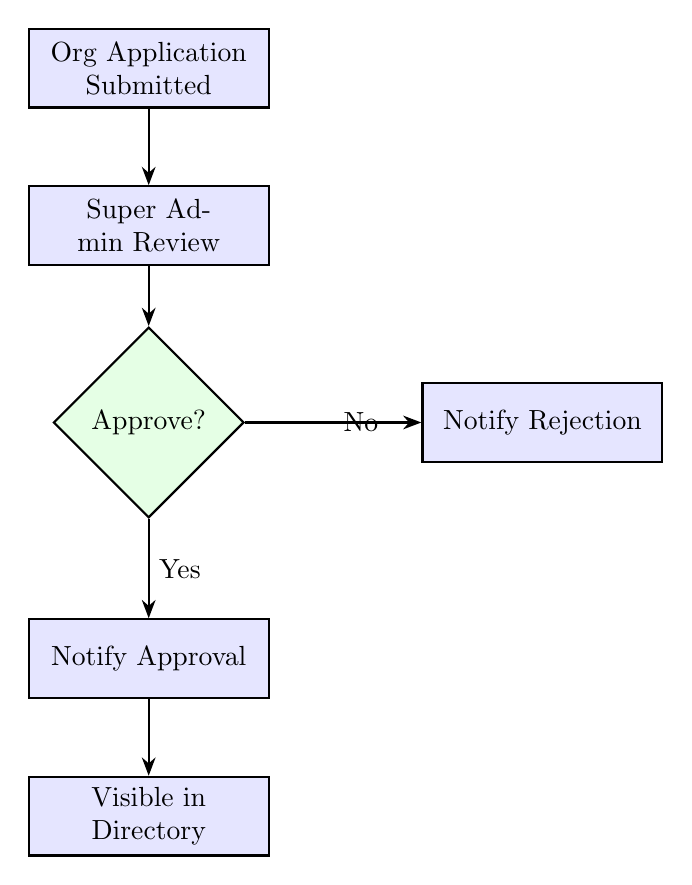
\begin{tikzpicture}[node distance=2cm, auto,
  process/.style={rectangle, draw=black, thick, fill=blue!10, text width=8em, text centered, minimum height=1cm},
  decision/.style={diamond, draw=black, thick, fill=green!10, text width=6em, text centered, inner sep=0pt},
  arrow/.style={thick, ->, >=Stealth}
]

\node (app) [process] {Org Application Submitted};
\node (review) [process, below of=app] {Super Admin Review};
\node (decide) [decision, below of=review, yshift=-0.5cm] {Approve?};
\node (reject) [process, right of=decide, xshift=3cm] {Notify Rejection};
\node (notify) [process, below of=decide, yshift=-1cm] {Notify Approval};
\node (visible) [process, below of=notify] {Visible in Directory};

\draw [arrow] (app) -- (review);
\draw [arrow] (review) -- (decide);
\draw [arrow] (decide) -- node[right] {No} (reject);
\draw [arrow] (decide) -- node[right] {Yes} (notify);
\draw [arrow] (notify) -- (visible);

\end{tikzpicture}
\caption{Approval Workflow Diagram}
\end{figure}

\section{Live Notification Flow}

\begin{figure}[h]
\centering
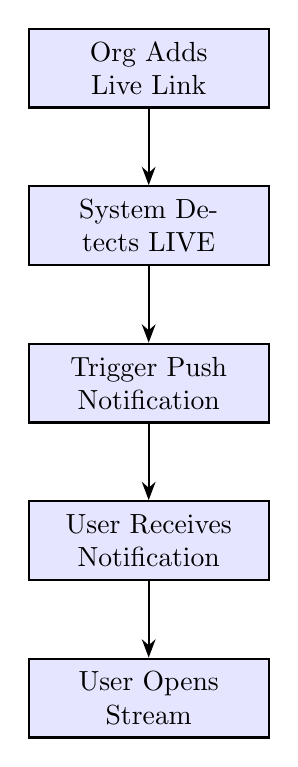
\begin{tikzpicture}[node distance=2cm, auto,
  process/.style={rectangle, draw=black, thick, fill=blue!10, text width=8em, text centered, minimum height=1cm},
  decision/.style={diamond, draw=black, thick, fill=green!10, text width=6em, text centered, inner sep=0pt},
  arrow/.style={thick, ->, >=Stealth}
]

\node (add) [process] {Org Adds Live Link};
\node (detect) [process, below of=add] {System Detects LIVE};
\node (trigger) [process, below of=detect] {Trigger Push Notification};
\node (receive) [process, below of=trigger] {User Receives Notification};
\node (open) [process, below of=receive] {User Opens Stream};

\draw [arrow] (add) -- (detect);
\draw [arrow] (detect) -- (trigger);
\draw [arrow] (trigger) -- (receive);
\draw [arrow] (receive) -- (open);

\end{tikzpicture}
\caption{Live Notification Flow Diagram}
\end{figure}

% -------------------------------------------------------------------
% 9. System Architecture
% -------------------------------------------------------------------
\chapter{System Architecture}

\section{Frontend Architecture (Flutter)}
The mobile application is built using Google's Flutter framework. It utilizes the BLoC (Business Logic Component) or Riverpod pattern for state management, ensuring a reactive and testable UI.

\section{Backend Services (Firebase)}
The backend relies on Firebase's suite of serverless tools, providing a robust and maintenance-free infrastructure.

\section{Clean Architecture}
The project is structured into three main layers:
\begin{itemize}
    \item \textbf{Presentation Layer:} UI widgets and state management logic.
    \item \textbf{Domain Layer:} Entities and business use cases (platform agnostic).
    \item \textbf{Data Layer:} Repositories, data sources, and models.
\end{itemize}

% -------------------------------------------------------------------
% 10. Technology Stack
% -------------------------------------------------------------------
\chapter{Technology Stack}

\begin{itemize}
    \item \textbf{Frontend Framework:} Flutter (Dart)
    \item \textbf{Backend Platform:} Firebase
    \item \textbf{Database:} Cloud Firestore (NoSQL)
    \item \textbf{Authentication:} Firebase Auth
    \item \textbf{Storage:} Firebase Cloud Storage (Images/Media)
    \item \textbf{Notifications:} Firebase Cloud Messaging (FCM)
    \item \textbf{State Management:} Riverpod
\end{itemize}

% -------------------------------------------------------------------
% 11. Database Design
% -------------------------------------------------------------------
\chapter{Database Design}
The database utilizes Cloud Firestore's document-collection model.

\section{Collections}
\begin{itemize}
    \item \texttt{users}: Stores user profile data, role, and preferences.
    \item \texttt{organizations}: Stores extended profile data for orgs (location, description, live status).
    \item \texttt{posts}: Stores social feed content.
    \item \texttt{notifications}: Stores user alerts history.
    \item \texttt{relationships}: Tracks "following" status between users and organizations.
\end{itemize}

\section{NoSQL Justification}
Firestore was chosen for its flexibility, real-time synchronization capabilities, and ease of scaling, which aligns perfectly with the dynamic nature of a social feed and live status updates.

% -------------------------------------------------------------------
% 12. Security Design
% -------------------------------------------------------------------
\chapter{Security Design}
\begin{itemize}
    \item \textbf{Firestore Rules:} Granular security rules ensure users can only read/write data they are authorized to access.
    \item \textbf{Validation:} Input validation on both client and server sides prevents injection attacks.
    \item \textbf{Data Privacy:} Personal user data is protected and not exposed publicly without consent.
\end{itemize}

% -------------------------------------------------------------------
% 13. UI/UX Design Approach
% -------------------------------------------------------------------
\chapter{UI/UX Design Approach}

\section{Theme System}
The application supports both Light and Dark modes. The default theme utilizes a warm color palette (Coral Pink, Soft Peach, etc.) to evoke a welcoming community feel.

\section{Accessibility}
High contrast ratios, scalable text, and intuitive navigation patterns are implemented to maximize accessibility for all users.

% -------------------------------------------------------------------
% 14. Deployment & Scalability
% -------------------------------------------------------------------
\chapter{Deployment & Scalability}
The app is designed for cross-platform deployment to the Apple App Store and Google Play Store from a single codebase. The serverless backend scales automatically to handle traffic surges without manual intervention.

% -------------------------------------------------------------------
% 15. Revenue & Monetization Model
% -------------------------------------------------------------------
\chapter{Revenue & Monetization Model}
\begin{itemize}
    \item \textbf{Subscription Plans:} Premium tiers for organizations to access advanced analytics or priority listing.
    \item \textbf{Featured Listings:} Paid placement for organizations at the top of directory searches.
    \item \textbf{Sponsored Notifications:} Ability for organizations to send promoted messages to the community.
\end{itemize}

% -------------------------------------------------------------------
% 16. Future Enhancements
% -------------------------------------------------------------------
\chapter{Future Enhancements}
\begin{itemize}
    \item \textbf{Direct Messaging:} Real-time chat between users and organizations.
    \item \textbf{Advanced Analytics:} Dashboards for organizations to track engagement.
    \item \textbf{AI-Powered Recommendations:} Personalized content sourcing based on user behavior.
    \item \textbf{Web Admin Panel:} A dedicated web interface for Super Admins for easier management.
\end{itemize}

% -------------------------------------------------------------------
% 17. Conclusion
% -------------------------------------------------------------------
\chapter{Conclusion}
eDirectory represents a powerful tool for community building. By combining the essential utility of a directory with the engaging features of a modern social network, it provides a unique value proposition. The robust architecture and scalable technology stack ensure that the platform can grow with the community, providing a secure and reliable experience for years to come.

\end{document}
